\documentclass[]{standalone}
%\documentclass[dvisvgm]{minimal}

\usepackage[]{tikz}
\usepackage{sfmath}
\usepackage{amsmath, amsfonts}
\usepackage{enumitem}
\usepackage{pgfplots}
\pgfplotsset{compat=1.16}

\usetikzlibrary{positioning,arrows.meta}

\renewcommand{\familydefault}{\sfdefault}

\begin{document}
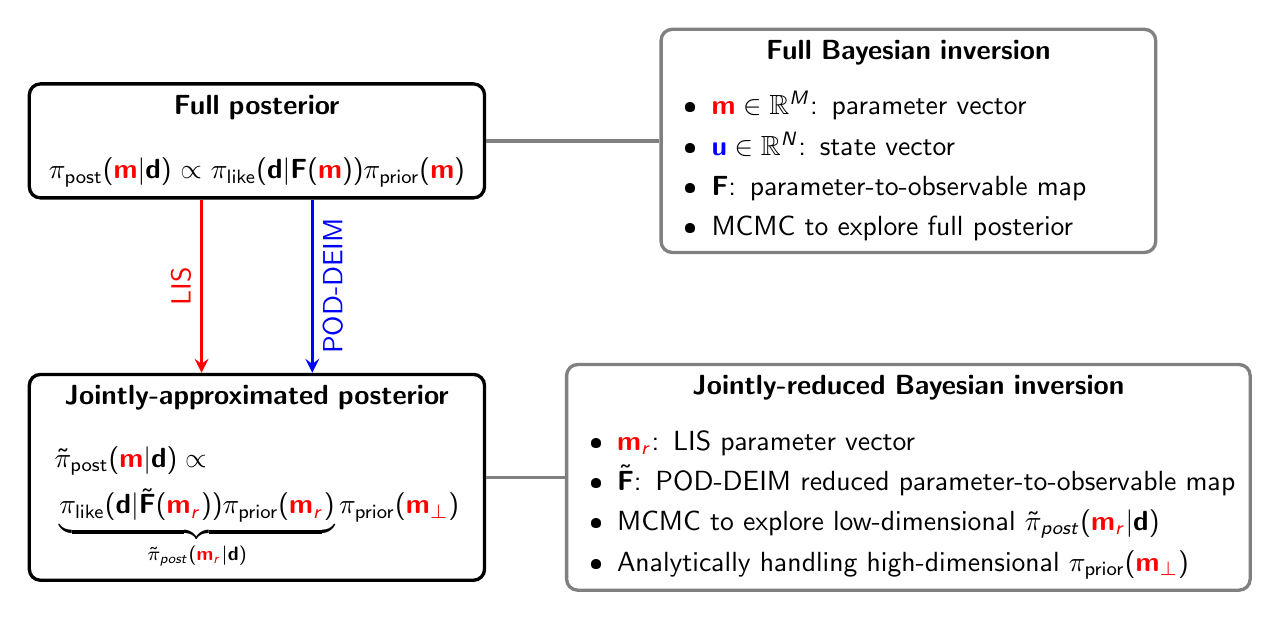
\begin{tikzpicture}[>=stealth]
  \node[inner sep=4pt, draw=black, very thick, rectangle, rounded corners,
    text centered, text width=5.5cm
    ]
    (full) {
      \textbf{Full posterior}\\
      \vspace{4mm}
      $\pi_\text{post}(\textcolor{red}{\mathbf{m}} | \mathbf{d}) \propto
      \pi_\text{like}(\mathbf{d}|\mathbf{F}(\textcolor{red}{\mathbf{m}}))
      \pi_\text{prior}(\textcolor{red}{\mathbf{m}})$
    };
  \node[inner sep=4pt, draw=black, very thick, rectangle, rounded corners,
    text centered, text width=5.5cm,
    below =2.2cm of full
    ]
    (reduced) {
      \textbf{Jointly-approximated posterior}
      \\
      \vspace{-4mm}
      \begin{align*}
        &\tilde{\pi}_\text{post} (\textcolor{red}{\mathbf{m}} | \mathbf{d})
        \propto \\
&\underbrace{\pi_\text{like}(\mathbf{d}|\tilde{\mathbf{F}}(\textcolor{red}{\mathbf{m}_r}))
\pi_\text{prior}(\textcolor{red}{\mathbf{m}_r})}_{\tilde{\pi}_{post}(\textcolor{red}{\mathbf{m}_r} | \mathbf{d})}
        \pi_\text{prior}(\textcolor{red}{\mathbf{m}_\perp})
      \end{align*}
    };

  \node [right=of reduced,
    inner sep=4pt, draw=gray, very thick, rectangle, rounded corners,
    text centered,
    text width=8.4cm] (reduced_bayesian) {
      \textbf{Jointly-reduced Bayesian inversion}
      \begin{itemize}[leftmargin=.5cm]
        \setlength\itemsep{-0.5mm}
        \item $\textcolor{red}{\mathbf{m}_r}$: LIS parameter vector
        \item $\tilde{\mathbf{F}}$: POD-DEIM reduced parameter-to-observable map
        \item MCMC to explore low-dimensional
          $\tilde{\pi}_{post}(\textcolor{red}{\mathbf{m}_r} | \mathbf{d})$
        \item Analytically handling high-dimensional
          $\pi_\text{prior}(\textcolor{red}{\mathbf{m}_\perp})$
      \end{itemize}
    };

  \node [
    inner sep=4pt, draw=gray, very thick, rectangle, rounded corners,
    text centered,
    text width=6cm] (full_bayesian)
    at (full.east -| reduced_bayesian.north)
    {
      \textbf{Full Bayesian inversion}
      \begin{itemize}[leftmargin=.5cm]
        \setlength\itemsep{-0.5mm}
        \item $\textcolor{red}{\mathbf{m}} \in \mathbb{R}^M$: parameter vector
        \item $\textcolor{blue}{\mathbf{u}} \in \mathbb{R}^N$: state vector
        \item $\mathbf{F}$: parameter-to-observable map
        \item MCMC to explore full posterior
      \end{itemize}
    };


  \path [very thick] ([xshift=-2em] reduced.north) edge [<-,red]
    node[sloped,above]{LIS} ([xshift=-2em] full.south)
    ([xshift=2em] reduced.north) edge [<-,blue]
    node[sloped,below]{POD-DEIM} ([xshift=2em] full.south);

  \path [very thick] (full.east) edge [-,gray] (full_bayesian.west)
    (reduced.east) edge [-,gray] (reduced_bayesian.west);


\end{tikzpicture}
\end{document}
